% Head
\documentclass[professionalfont]{beamer}
%\documentclass{beamer}
\usetheme{Berkeley}
\usecolortheme{default}

%Information to be included in the title page:
\usepackage{amsthm,amssymb,amsmath,mathrsfs,graphicx,xcolor,float,url}


%%%%%%%%%%%%%%%%%%%%%%%%
\usepackage{tkz-tab,tikz,fancyhdr}
\usetikzlibrary{decorations.markings}
%\tikzstyle{vertex}=[circle, draw, inner sep=0pt, minimum size=5pt]
%%%%%%%%%%%%%%%%%%%%%%%%%%%%
\usetikzlibrary{arrows}
\usepackage{pgfplots}
\usetikzlibrary{snakes}
%%%%%%%%%%%%%%%%%%%%



\usepackage{ifthen}
%\usepackage[pagebackref=false,colorlinks,linkcolor=black,citecolor=magenta]{hyperref}
\usepackage{calc}
%\usepackage[pagebackref=false,colorlinks,linkcolor=blue,citecolor=magenta]{hyperref}

% Mine
\usepackage[numbers,sort&compress]{natbib}
\usepackage{caption}
\usepackage{wrapfig}
\usepackage{blindtext}
\usepackage{etoolbox}
\usepackage{times}

%برخی از دستورات از قبیل تعریف اندازه متن، فراخوانی پکیج‌ها، فراخوانی زیپرشین و تعریف فونت‌ها و 
%چند دستور دیگر در  فایل   head (در دستور بالا)  قرار دارد. در صورت نیاز می‌توان آنرا تغییر داد 
% حتما باید فونت‌های زیر برروی کامپیوتر شما نصب شده باشد: Parsi Digits،  Yas،  IranNastaliq
% ==========+==========#==========+==========#==========+==========#==========+==========#==========+==========
% دستورات خاصی که میتوانند کمک‌کننده باشند

% دستور علامت درصد
\newcommand{\perc}{ \hspace*{-3mm} { \percentfont \textbf{\%} } \hspace*{-2.5mm} }

% دستور چاپ علامت / برای موقعی که یک طرف عدد نباشد و علامت / چاپ نشود!
\newcommand{\dpt}{{}_\textbf{\texttt{/}}}

%\renewcommand{\arraystretch}{1.1}
% =========+=========+=========+=========+=========+=========+========= Other
\newcommand{\mycomment}[1]{}
\newcommand{\warning}[1]{\textcolor{red}{\textbf{#1}}}

% label
\numberwithin{equation}{chapter}
%\numberwithin{equation}{section}

% section
\setcounter{tocdepth}{5}
\setcounter{secnumdepth}{5}

% shape
%\DeclareCaptionLabelSeparator{none}{ }
%\captionsetup{labelsep=none}

% =========+=========+=========+=========+=========+=========+========= Symbols

\newcommand{\allrights}{\tiny{\ \circledR}}
%\scriptsize{\textcircled{\tiny{R}}}

% =========+=========+=========+=========+=========+=========+========= textup
\newcommand{\efn}[1]{\LTRfootnote{\lr{\textup{#1}}}}
\newcommand{\eng}[1]{\lr{\textup{#1}}}
\newcommand{\per}[1]{\text{\rl{#1}}}
\newcommand{\codd}[1]{\lr{\texttt{\textup{#1}}}}
\newcommand{\cod}[1]{\lr{\texttt{\textup{\detokenize{#1}}}}}
\newcommand{\codb}[1]{\textbf{\lr{\texttt{\textup{\detokenize{#1}}}}}}

% =========+=========+=========+=========+=========+=========+========= cod
\newenvironment{code}{\latin \Verbatim[tabsize=4, baselinestretch=1, fontshape=normal]}{\endVerbatim \endlatin} 

\newenvironment{file}[1]{$\ $ \newline \\ \minipage{16cm} \latin \fbox{\cod{#1}} \vspace{-2mm} \Verbatim[tabsize=4, baselinestretch=1, fontshape=normal, frame=single]}{\endVerbatim \endlatin \endminipage \\ $\ $ \\} 

\newenvironment{terminal}{$\ $ \newline \\ \minipage{16cm} \latin \centering{\fbox{\cod{Terminal}}} \vspace{-3mm} \Verbatim[tabsize=4, baselinestretch=1, fontshape=normal, frame=single]}{\endVerbatim \endlatin \endminipage \\ $\ $ \\} 

\newcommand{\myspace}{\vspace{-1cm}} % reduce vspace between two minipage 
\newcommand{\halfspace}{\vspace{-1.5cm}} % reduce vspace between two minipage 
\newcommand{\somespace}{\vspace{-2cm}} % reduce vspace some where 

\AfterEndEnvironment{code}{\noindent\ignorespaces}
\AfterEndEnvironment{file}{\noindent\ignorespaces}
\AfterEndEnvironment{terminal}{\noindent\ignorespaces}
\AfterEndEnvironment{con}{\noindent\ignorespaces}

% =========+=========+=========+=========+=========+=========+========= space after
\setlength{\parindent}{0pt}
\mycomment{
\AfterEndEnvironment{theorem}{\noindent\ignorespaces}
\AfterEndEnvironment{corollary}{\noindent\ignorespaces}
\AfterEndEnvironment{definition}{\noindent\ignorespaces}
\AfterEndEnvironment{example}{\noindent\ignorespaces}
\AfterEndEnvironment{lemma}{\noindent\ignorespaces}
\AfterEndEnvironment{note}{\noindent\ignorespaces}
\AfterEndEnvironment{proposition}{\noindent\ignorespaces}
\AfterEndEnvironment{remark}{\noindent\ignorespaces}
\AfterEndEnvironment{proof}{\noindent\ignorespaces}
\AfterEndEnvironment{table}{\noindent\ignorespaces}
\AfterEndEnvironment{latin}{\noindent\ignorespaces}
}


% Commands

% Comment
\newcommand{\mycomment}[1]{}

% Shape
\newcommand{\tikzci}{\tikz[baseline=-0.5ex]\draw[black,fill=black,radius=5pt] (0,0) circle ;}%


% Symbol
\newcommand{\taualpha}{\tau ^{-\alpha}}
\newcommand{\taugamma}{\frac{\tau ^{-\alpha}}{\Gamma(2-\alpha)}}
\newcommand{\pap}{(\alpha)}
\newcommand{\Ne}{N_{exp}}
\newcommand{\sltau}{s_{l} \tau}
\newcommand{\esltau}{e^{-s_{l} \tau}}
\newcommand{\C}{\mathbb{C}}
\newcommand{\R}{\mathbb{R}}
\newcommand{\D}{\mathbb{D}}
\newcommand{\tD}{\tilde{\mathbb{D}}}
\newcommand{\U}{\mathcal{U}}
\newcommand{\bpo}{\Big{(}}
\newcommand{\bpc}{\Big{)}}

% Operator
\newcommand \inner[2] { \langle #1, #2 \rangle }
\newcommand \norm[1] { \parallel #1 \parallel }

\newcommand \difbeta[1]
{{
\dfrac{\partial^{\beta} #1}{\partial |x|^{\beta}}
}}
\newcommand \difbetal[1]
{{
_{a}D_{x}^{\beta} #1
}}
\newcommand \difbetar[1]
{{
_{x}D_{b}^{\beta} #1
}}
\newcommand \diffbeta[1]
{{
\dfrac{\partial^{2 \beta} #1}{\partial |x|^{2 \beta}}
}}
\newcommand \diffbetal[1]
{{
_{a}D_{x}^{2 \beta} #1
}}
\newcommand \diffbetar[1]
{{
_{x}D_{b}^{2 \beta} #1
}}

% Space
\newcommand{\stq}{(\star) \quad}
\newcommand{\sts}{(\star) \ }
\newcommand{\srs}{\  \rightarrow \ }
\newcommand{\qrq}{\quad \rightarrow \quad}
\newcommand{\qcq}{\quad , \quad}

% Number
\addtobeamertemplate{navigation symbols}{}
{%
\usebeamerfont{footline}%
\usebeamercolor[fg]{footline}%
\hspace{1em}%
\insertframenumber/\inserttotalframenumber
}

% Label
\DeclareCaptionLabelSeparator{none}{}
%\captionsetup{labelsep=none}
% ==========+==========#==========+==========#==========+==========#==========+==========#==========+==========
% ==========+==========#==========+==========#==========+==========#==========+==========#==========+==========
% ==========+==========#==========+==========#==========+==========#==========+==========#==========+==========
% اطلاعات زیر را تکمیل کنید
% ==========+==========#==========+==========#==========+==========#==========+==========#==========+==========
\besmella{156}  %{انتخاب لوگوی بسم‌الله الرحمن الرحیم}%  besmellah or from  besmellah-0 to besmellah-7
\university{دانشگاه صنعتی اصفهان}
\department{دانشکده علوم ریاضی}
\Sdegree{ریاضی کاربردی}
\gender{آقای} %جنسیت
\name{علی فروزنده هفشجانی}
\Ename{Ali Forouzandeh Hafshejani}
\SetDegree{2} % مقطع
% 1 B.Sc. 
% 2 M.Sc. 
% 3 Ph.D.
\yearr{1403}
\timeofmeeting{شنبه 10/06/1403 ساعت 30:10}
\dateofmeeting{10 شهریور 1403}
\Edate{31/8/2024} %{تاریخ دفاع}
\EdateB{August 2024} %{تاریخ دفاع}
\placeofmeeting{سالن خوارزمی دانشکده‌ علوم ریاضی} 
\Title{الگوریتم‌های کاهش در زمان چندشبکه‌ای برای حل معادلات با مشتقات جزئی کسری}
\Etitle{Multigrid reduction-in-time algorithms for solving fractional partial differential equations}
% ==========+==========#==========+==========#==========+==========#==========+==========#==========+==========
% ==========+==========#==========+==========#==========+==========#==========+==========#==========+==========
% ==========+==========#==========+==========#==========+==========#==========+==========#==========+==========
\supervisor{دکتر رضا مختاری}
% نام و نام خانوادگی استاد راهنما را به فارسی در خط بالا بیاورید
\Esupervisor{Dr. Reza Mokhtari}
\supervisordegree{Professor} 
  %{نام و نام خانوادگی استاد راهنما به انگلیسی  و درجه‌ی علمی او  را در خط بالا بیاورید}
% ==========+==========#==========+==========#==========+==========#==========+==========#==========+==========
\supervisorB{}
% نام و نام خانوادگی استاد راهنمای دوم را به فارسی در خط بالا بیاورید.  اگر استاد راهنمای دوم ندارید بین دو آکولاد را خالی کنید
\EsupervisorB{}
\supervisorBdegree{} 
% نام و نام خانوادگی استاد راهنمای دوم به انگلیسی  و درجه‌ی علمی او  را در خط بالا بیاورید. اگر استاد راهنمای دوم ندارید بین دو آکولاد را خالی کنید
% ==========+==========#==========+==========#==========+==========#==========+==========#==========+==========
\advisor{دکتر محدثه رمضانی}
%% نام و نام خانوادگی استاد مشاور به فارسی.  اگر استاد مشاور ندارید بین دو آکولاد را خالی کنید
\Eadvisor{Dr. Mohadese Ramezani}
%% نام و نام خانوادگی استاد مشاور به انگلیسی.  اگر استاد مشاور ندارید بین دو آکولاد را خالی کنید
\advisordegree{Postdoctoral}
%{درجه علمی استاد مشاور}
% ==========+==========#==========+==========#==========+==========#==========+==========#==========+==========
\refereeA{دکتر هادی روحانی}
\refereeAUniversity{دانشگاه صنعتی مالک اشتر}
% نام و نام خانوادگی داور اول به فارسی  و دانشگاه او. اگر داور اول داخل دانشکده است بین دو آکولاد را خالی کنید
\ErefereeA{Dr. Haadi Rouhani}\refereeAdegree{Associate Professor}    
% نام و نام خانوادگی داور اول به انگلیسی و درجه علمی او. اگر داور اول داخل دانشکده است بین دو آکولاد را خالی کنید
% ==========+==========#==========+==========#==========+==========#==========+==========#==========+==========
\refereeB{دکتر مریم محمدی}
\refereeBUniversity{دانشگاه خوارزمی}
% نام و نام خانوادگی داور دوم به فارسی  و دانشگاه او. اگر داور دوم داخل دانشکده است بین دو آکولاد را خالی کنید
\ErefereeB{Dr. Maryam Mohammadi}\refereeBdegree{Associate Professor}    
% نام و نام خانوادگی داور دوم به انگلیسی و درجه علمی او. اگر داور دوم داخل دانشکده است بین دو آکولاد را خالی کنید
% ==========+==========#==========+==========#==========+==========#==========+==========#==========+==========
\refereeC{}
\refereeCUniversity{}
% نام و نام خانوادگی داور دوم به فارسی  و دانشگاه او. اگر داور سوم ندارید بین دو آکولاد خالی باشد
\ErefereeC{}\refereeCdegree{}
% نام و نام خانوادگی داور سوم به انگلیسی و درجه علمی او. اگر داور سوم ندارید بین دو آکولاد خالی باشد
% ==========+==========#==========+==========#==========+==========#==========+==========#==========+==========
\coordinator{دکتر محمود بهبودی}
\Ecoordinator{Dr. Mahmood Behboodi}
\coordinatordegree{Professor}      
%سرپرست تحصیلات تکمیلی دانشکده و درجه علمی او
% ==========+==========#==========+==========#==========+==========#==========+==========#==========+==========
\Euniversity{Isfahan University of Technology}
\Edepartment{Department of Mathematical Sciences}
% ==========+==========#==========+==========#==========+==========#==========+==========#==========+==========
% ==========+==========#==========+==========#==========+==========#==========+==========#==========+==========
% ==========+==========#==========+==========#==========+==========#==========+==========#==========+==========
%چکیده سخنرانی که در جلسه دفاع از پایان نامه ارائه خواهد شد، اینجا بیاید
% ==========+==========#==========+==========#==========+==========#==========+==========#==========+==========
\talkabstract{\small
در سال‌های اخیر، معادلات دیفرانسیل با مشتقات کسری نقش بسیار مهمی در مدل‌سازی ریاضی بسیاری از مسائل دنیای واقعی ایفا کرده‌اند.
علت اصلی این است که مشتقات کسری بر خلاف مشتقات مرتبه صحیح موضعی نبوده و از اطلاعات بیشتری استفاده می‌کنند.
معادلات انتشار کسری‑مکانی، یک دسته مهم از این معادلات هستند که برای مدل‌سازی پدیده‌های انتشار (زیرانتشار/زبرانتشار) کاربرد فراوانی دارند.
در این پایان‌نامه، پس از مرور مفاهیم مورد نیاز از آنالیز تابعی و حسابان کسری، برخی از فضاهای کسری و ویژگی‌های آن‌ها بررسی شده‌اند.
در ادامه، یک مسئله انتشار کسری‑مکانی با شرایط مرزی دیریکله بیان شده و با استفاده از روش عناصر متناهی با گسسته‌سازی مکانی‑زمانی، یک حلقه پیشروی زمانی برای حل عددی آن ساخته شده است که در هر گام زمانی، یک دستگاه در بعد مکانی حل می‌شود.
این حلقه پیشرو زمانی با یک دستگاه بلوکی دوقطری معادل شده که حل این دستگاه بزرگ در بعد زمانی انجام می‌شود.
در پایان پس از مرور سریع روش‌های موازی‌سازی در زمان، یک نسخه دوسطحی از روش کاهش در زمان چندشبکه‌ای برای حل دستگاه بلوکی دوقطری به ‌کار برده شده و آنالیز همگرایی آن بررسی می‌شود.
\vdots \vdots \vdots
\\
\textbf{واژگان کلیدی:}
حسابان کسری،‌ معادلات انتشار کسری-مکانی، روش عناصر متناهی، موازی‌سازی در زمان، روش کاهش در زمان چندشبکه‌ای.
}
% ==========+==========#==========+==========#==========+==========#==========+==========#==========+==========
% ==========+==========#==========+==========#==========+==========#==========+==========#==========+==========
% ==========+==========#==========+==========#==========+==========#==========+==========#==========+==========
\taghdim{
\begin{Huge}
\begin{flushright}\hspace{1cm}  \vspace{1cm}
تقدیم به
\\
\begin{center}
\bf{فروزندگان راه تاریک علم؛}
\\
\end{center}
\end{flushright}
\vspace{1cm}
\begin{flushleft}
آنان که برای بیداری انسان از خواب غفلت، رویاها و زندگی خود را فدا کردند.
\end{flushleft}
\end{Huge}
}
\Thanks{
\begin{huge}
\begin{tabular}{l c c c r}
به نام خداوند جان و خرد
&&&&
کز این برتر اندیشه بر نگذرد
\\
خداوند نام و خداوند جای
&&&&
خداوند روزی‌ده رهنمای
\\
خداوند کیوان و گردان‌سپهر
&&&&
فروزنده ماه و ناهید و مهر
\\
ز نام و نشان و گمان برتر است
&&&&
نگارنده برشده پیکر است
\\
به بینندگان آفریننده را
&&&&
نبینی مرنجان دو بیننده را
\\
نیابد بدو نیز اندیشه راه
&&&&
که او برتر از نام و از جایگاه
\end{tabular}
\\
\qquad\qquad\qquad\qquad\qquad\qquad
- فردوسی
\begin{flushright}
در آغاز، بر خود لازم می‌دانم که از زحمات بی‌دریغ و راهنمایی‌های حکیمانه استاد راهنمای گرانقدر، جناب آقای دکتر رضا مختاری در راستای انجام این رساله تشکر و قدردانی نمایم.
بی‌شک همراهی خاضعانه ایشان در طول دوره کارشناسی تا کارشناسی ارشد سزاوار سپاسی بیش از این است.
از خانم دکتر محدثه رمضانی که امر مشاوره این پایان‌نامه را به عهده داشتند، بسیار متشکرم.
همچنین از داوران گرامی، آقای دکتر هادی روحانی و خانم دکتر مریم محمدی کمال سپاس و امتنان را دارم.
\\
از پدر و مادر مهربان و عزیزم، برادرم ایلیا و خواهرم شهربانو که همواره مشوق و حامی من در سختی‌ها و دشواری‌های زندگی بوده‌ند، کمال تشکر را دارم.
در پایان از تمامی استادان و دوستان، از جمله آقایان دکتر سید محمود منجگانی و دکتر فرید بهرامی، که در طول سالیان تحصیلی همواره در کنار من بوده‌اند و تجربه‌های ارزنده‌ای به اینجانب آموخته‌اند، بسیار سپاس گزارم.
\end{flushright}
\begin{flushleft}
علی فروزنده هفشجانی 
\large{04/06/1403}
\end{flushleft}
\end{huge}
}
% ==========+==========#==========+==========#==========+==========#==========+==========#==========+==========
% ==========+==========#==========+==========#==========+==========#==========+==========#==========+==========
% ==========+==========#==========+==========#==========+==========#==========+==========#==========+==========
% شروع متن 
\begin{document}
%%%%%%%%%%%%%%%%%%%%% Error at this line is because of Title in style.sty
\defpage   %{برای تولید اطلاعیه دفاع این دستور را فعال کنید}
\besmellapage  %{برای تولید صفحه بسم الله این دستور را فعال کنید}
\firstpage  %{ برای تولید صفحه اول پایان نامه این دستور را فعال کنید}
\approvalpage %{برای تولید صفحه صورتجلسه دفاعیه  این دستور را فعال کنید}
\thatkspage  %{برای تولید صفحه تشکر این دستور را فعال کنید}
\copyrightpagepage  %{برای تولید صفحه کپی رایت این دستور را فعال کنید}
\taghdimpage  %{برای تولید صفحه تقدیم این دستور را فعال کنید}
% ==========+==========#==========+==========#==========+==========#==========+==========#==========+==========
\setcounter{page}{7} %{تعداد صفحات قبل از فهرست مطالب را بشمارید  و این شمارنده را برابر عددی که  صفحه فهرست مطالب باشد قرار دهید }
\renewcommand{\thepage}{\adadi{page}}
\tableofcontents
\newpage
\pagestyle{empty}
\fancyhf{}
%%%%%%%%%%%%%%%%%%%%%%%%%%%%%%%%%%%%%%%%%%%%%%%%%%%%%%%%%%%%%%%%%%%
%%%%%%%%%%%%%%%%%%%%%%%%%%%%%%%%%%%%%%%%%%%%%%%%%%%%%%%%%%%%%%%%%%%
\vspace*{-1cm}                   %%%  فاصله را خودتان با توجه به حجم چکیده تنظیم کنید  
\thispagestyle{empty}
{\large\bf چکیده: }  
\vspace*{0.1cm}
\\
{\small
امروزه معادلات دیفرانسیل جزئی کسری
(\eng{FPDE})
کاربردهایی در مسائل دنیای واقعی در حوزه‌های علوم و مهندسی پیدا کرده‌اند.
این محبوبیت از ویژگی غیرموضعی مشتق کسری در مقایسه با ماهیت موضعی بودن مشتق مرتبه صحیح نتیجه می‌شود.
یکی از مهم‌ترین
\eng{FPDE}ها،
معادله انتشار کسری-مکانی
(\eng{SFD})
است که در مدل‌سازی انتشار غیرعادی، بررسی پدیده‌های زیرانتشار و توصیف دینامیک‌های آشوبی کاربرد دارد.
معادله
\eng{SFD}
با بعد دو مکانی به‌عنوان یک معادله انتشار کلیدی شناخته می‌شود.
این معادلات از تعمیم مشتقات مکانی مرتبه صحیح به مرتبه کسری در معادله دیفرانسیل مشتقات جزئی حاصل می‌شود.
از آنجا که اکثر معادلات 
\eng{SFD}
به‌صورت تحلیلی قابل حل نیستند، روش‌های عددی مختلفی مانند روش تفاضل متناهی، رویکرد گالرکین ناپیوسته موضعی و روش عناصر متناهی (FEM) برای دستیابی به دقت و کارایی بالا پیشنهاد شده‌اند.
با توجه به این نکته که مشتقات کسری برخلاف مشتقات صحیح غیرموضعی هستند.
در نتیجه صرف نظر از روش گسسته‌سازی مورد استفاده، حجم زیادی از محاسباتی به دلیل غیرموضعی بودن عملگرهای دیفرانسیل کسری مورد نیاز است.
بسیاری از محققان بر روی توسعه الگوریتم‌های سریع برای مقابله با این چالش کار کرده‌اند.
علاوه بر این راه‌حل‌های سریع، رویکردهای محاسباتی موازی مانند کاهش در زمان چندشبکه‌ای
(\eng{MGRIT})
نیز باید به‌عنوان روش‌های مؤثر در نظر گرفته شوند.
در این پایان‌نامه، با بحث در مورد مفاهیم اساسی در آنالیز تابعی، از جمله فضاهای برداری، فضاهای تابع و فضاهای سوبولف و همچنین اصول حسابان کسری شروع می‌کنیم و توضیح می‌دهیم که مشتق‌ها و انتگرال‌های کسری، پایه‌های حسابان کسری هستند و مشتق کسری ریس به‌طور مخصوص برای کاربردهای حوزه مکانی مورد علاقه است.
در ادامه فضاهای کسری مختلف مانند فضاهای سوبولف کسری را بیان کرده و خواص آن‌ها را بررسی می‌کنیم و به فضاهای مرتبط با
\eng{FPDE}ها
نیز اشاره می‌کنیم.
پس از آن، مسئله
\eng{SFD}
را با شرایط مرزی دیریکله بررسی می‌کنیم.
حال
\eng{FEM} 
را بیان کرده و خواص آن را توضیح می‌دهیم.
سپس شکل ضعیف معادله
\eng{SFD}
را می‌سازیم و گسسته‌سازی مکانی-زمانی را با استفاده از گسسته‌سازی مکانی یکنواخت و گسسته‌سازی زمانی غیریکنواخت اعمال می‌کنیم.
این فرایند موجب تولید یک دستگاه بزرگ و تنک از معادلات می‌شود.
برای حل عددی معادله
\eng{SFD}،
روش را به‌عنوان یک حلقه پیشرو زمانی نشان می‌دهیم که در آن یک دستگاه خطی در بعد مکانی در هر مرحله زمانی حل می‌شود.
این حلقه پیشرو زمانی به‌عنوان یک روش تک‌گامی در زمان نیز عمل می‌کند و معادل با حل یک دستگاه بلوکی دوقطری پایین مثلثی در بعد زمان است. 
پس روش‌های مختلفی را برای موازی‌سازی زمانی مورد بحث قرار می‌دهیم و یک تاریخچه مختصر ارائه می‌کنیم.
یکی از روش‌های قابل توجه،
\eng{MGRIT} 
است که از رویکرد کاهش چندشبکه‌ای استفاده می‌کند. 
روش
\eng{MGRIT}
دو مزیت قابل توجه دارد: استقلال نسبی از کدهای موجود و مقیاس‌بندی الگوریتمی بهینه.
در ادامه، از نسخه دوسطحی
\eng{MGRIT}
برای حل آن دستگاه بلوکی دوقطری پایین مثلثی استفاده کرده و به تحلیل عملکرد همگرایی روش می‌پردازیم. 
در نهایت یک مثال عددی را در
\Matlab
و
\XBraid
پیاده‌سازی کرده و عملکرد روش‌های عددی را بررسی می‌کنیم.
نتایج نشان می‌دهد که روش سازگاری و همگرایی کافی را برای حل‌های عددی چنین معادلات
\eng{SFD}
نشان می‌دهد و می‌توان آن را برای حل برخی 
\eng{FPDE}‌های
پیچیده گسترش داد.
}
\\[.1cm]
{\bf رده‌بندی موضوعی:}
\lr{65M55, 65M60, 65Y05}\\[0.1cm]
  {\bf
 واژگان کلیدی:
 }
حسابان کسری،‌ معادلات انتشار کسری-مکانی، روش عناصر متناهی، موازی‌سازی در زمان، روش کاهش در زمان چندشبکه‌ای.
\newpage
% ==========+==========#==========+==========#==========+==========#==========+==========#==========+==========
\chapter*{پیشگفتار}
\addcontentsline{toc}{chapter}{پیشگفتار}
\thispagestyle{empty}
% ==========+==========+==========+==========+==========
یک دسته از معادلات انتشار پرکاربرد، معادله پخش گرما در بعد دو مکانی است که با تعمیم مشتقات مکانی مرتبه صحیح به مرتبه کسری، معادله انتشار کسری-مکانی
(\eng{SFD})
دوبعدی به دست می‌آید.
از آنجا که بیشتر معادلات
\eng{SFD}
را نمی‌توان به‌صورت دقیق (تحلیلی) حل کرد، روش‌های عددی متفاوت مانند تفاضلات متناهی
\cite{Ref4DXL, Ref9HFCS, Ref14FZLTAL, Ref15CDL}،
عناصر متناهی
\cite{Ref21BTY, Ref24BTWY, Ref25YYNWZL, Ref26ZBZT, Ref28BSYXZ}،
حجم متناهی
\cite{Ref30LZTBA, Ref31JW}
و طیفی
\cite{Ref33SX, Ref34Y}
برای دستیابی به دقت و کارایی بالا به‌طور گسترده مطرح شدند؛ اما به‌علت غیرموضعی بودن عملگرهای دیفرانسیل کسری، کار محاسباتی فشرده‌ای در کنار نوع گسسته‌سازی اعمال‌شده مورد نیاز است
\cite{Ref42GBTJL}.
به همین دلیل بسیاری از پژوهشگران سعی کرده‌اند الگوریتم‌های سریع مناسبی را برای مقابله با این چالش شناسایی کنند
\cite{Ref43PS, Ref48CLZ}.
به‌علاوه می‌توان از محاسبات موازی به‌عنوان یک راهبرد اساسی استفاده کرد.
گونگ\efn{Gong}
و همکاران الگوریتم‌های موازی بر پایه پردازنده و گرافیک رایانه را برای معادلات
\eng{SFD}
يک‌‌بعدی با مشتق کسری
ریس\efn{Riesz}
ارائه کردند
\cite{Ref49GBT, Ref50WLGZX}
که افزایش سرعت‌ آن با موازی‌سازی مکانی همراه با رویکرد گام‌های زمانی متوالی، با استفاده از انتشاردهنده زمان برای ادغام از یک زمان به زمان دیگر به ‌دست‌ می‌آید.
با این ‌حال برای افزایش سرعت محاسبات در آینده، باید به تعداد پردازنده‌های بیشتر به‌جای پردازنده‌های سریع‌تر تکیه کرد.
پس می‌توان نتیجه گرفت که الگوریتم‌های حل‌کننده محدود به موازی‌سازی مکانی برای مسائل دارای رفتار تکاملی، مستلزم زمان محاسباتی طولانی هستند و اغلب برای حل معادلات
\eng{SFD}
چندبعدی نیازمند منابع محاسباتی فراتر از منابع موجود هستند.
\\
اگرچه زمان به‌طور ذاتی متوالی است اما فن ﻣﻮﺍﺯﯼﺳﺎﺯﯼ ﺩﺭ ﺯﻣﺎﻥ، یک روش ﺟﺪﯾﺪ نیست و الگوریتم‌های دارای این فن، از تقاضای بالایی در ده سال اخیر برخوردار بوده‌اند.
در حال حاضر الگوریتم‌های فراواقعی در زمان
\cite{Ref51LMT}
و کاهش در زمان چندشبکه‌ای
(\eng{MGRIT})
\cite{Ref52FFKMS}
دو مورد مؤثر هستند.
وو\efn{Wu}
و
ژو\efn{Zhou}
خواص همگرایی الگوریتم فراواقعی را برای معادلات
\eng{SFD}
از طریق معادلات دیفرانسیل معمولی در گام‌ زمانی ثابت تجزیه و تحلیل کردند
\cite{Ref54WZ}،
اما آزمایشات در مقیاس بزرگ ارائه نشده‌ است.
با توجه به‌ این‌ که الگوریتم فراواقعی را می‌توان به‌عنوان نسخه دوسطحی روش کاهش چندشبکه‌ای تفسیر کرد
\cite{Ref52FFKMS, Ref55GV}،
همروندسازی آن به دلیل حل شبکه درشت متوالی بزرگ هنوز محدود است.
\\
یکی از مراجع مهمی که در تهیه این پایان‌نامه از آن استفاده شده، مقاله یو و همکاران
\cite{Ref0YSXBP}
است.
اکثر مطالب این پایان‌نامه بر سه موضوع حسابان کسری، روش عناصر متناهی و روش کاهش در زمان چندشبکه‌ای تمرکز دارند.
در فصل اول به مرور مفاهیم مقدماتی از آنالیز تابعی و آشنایی کافی با حسابان کسری پرداخته شده است.
همچنین فضاهای کسری مورد نیاز همراه با ویژگی‌های مهم آنان در این فصل بررسی شده‌اند.
سپس مسئله
\eng{SFD}
مورد نظر پایان‌نامه در شروع فصل دو بیان شده و پس از بازگویی
\eng{FEM}،
از آن جهت گسسته‌سازی مسئله
\eng{SFD}
مورد نظر و ساخت یک حلقه پیشرو زمانی استفاده شده است.
در نهایت جهت سرعت بخشیدن به محاسبه حلقه پیشرو زمانی به‌دست‌آمده، روش
\eng{MGRIT}
بیان و آنالیز همگرایی نسخه دوسطحی آن بررسی شده است.
روش‌های عددی نیز با استفاده از نرم‌افزار
\Matlab
و بسته نرم‌افزاری
\XBraid
پیاده‌سازی شده که کدهای مربوط به پیاده‌سازی در پیوند زیر قابل مشاهده هستند.
\begin{center}
\href{https://github.com/aforouz/Research_Papers/tree/main/MSc_Thesis}{\cod{https://github.com/aforouz/Research_Papers/tree/main/MSc_Thesis}}
\end{center}
در این پایان‌نامه، همه توابع حقیقی مقدار هستند.
همچنین ناحیه مستطیلی
$\Omega = (a, b) \times (c, d)$
که
$a,b,c,d \in \Real$،
به‌عنوان دامنه مکانی دوبعدی در نظر گرفته شده و تمامی تعریف‌ها براساس آن ارائه شده‌اند.
\clearpage
\pagestyle{fancy}
\fancyhf{}
\fancyhead[LO]{\nouppercase\rightmark\ \hfill\ \thepage}
\pagenumbering{arabic}
% ==========+==========#==========+==========#==========+==========#==========+==========#==========+==========
% Chapter 1
% Introductions and definitions 

% ==================== Introduction ====================

\section{Introduction}

% ====================Motivations==================

\subsection{Motivation}

\begin{frame}

\frametitle{Motivation}
\[
\frac{\mathrm{d^2} y}{\mathrm{d} t^2}+Ay= 0 ,\quad y(0) = y_0, \quad y^{'}(0) = y^{'}_0,
\]
$y(t) = cos(\sqrt{A}t)y_0 + (\sqrt{A})^{-1}sin(\sqrt{A}t)y^{'}_0 ,$
\newline
\newline
\[
A = \begin{pmatrix}
    -2 & 0 & 1 \\
     3 & 1 & -3 \\
     2 & 1 & 1
\end{pmatrix}
\quad \quad 
X^2 = A \quad X = ?
\]  
\newline
\newline

How "funm" and other functions in MATLAB work?
\end{frame}

% ==================== Definitions ====================

\subsection{Jordan Canonical Form}

% ====================JCF1=======================

\begin{frame}

\frametitle{Definitions \newline 1.Jordan Canonical Form}
There are many equivalent ways of defining $f(A)$.\newline
It is a standard result that any matrix $A \in C^{n \times n}$ can be expressed in the Jordan
canonical form. \newline

\[
Z^{-1}AZ = J = diag(J_{1},J_{2},...,J_{p}),\newline
\]

\[
J_{k}= \begin{pmatrix}
    \lambda_{k} & 1 & \\
      & \lambda_{k} &1& \\
     &  & \lambda_{k} &1 & \\
     & & & \lambda_{k} &1 & \\
     &&&&...&... \\
     &&&&&...
\end{pmatrix} \in C^{m_{k} \times m_{k} } ,
\]

\end{frame}

% ====================JCF2======================

\begin{frame}

\frametitle{Definitions \newline 1.Jordan Canonical Form}

\[
A = \begin{pmatrix}
    5 & 4 & 2 & 1 \\
    0 & 1 &-1 & -1 \\
    -1 & -1 &3 &0  \\
    1 &1 &-1 &2
    \end{pmatrix},\newline 
\]

\[
\chi(\lambda) = (\lambda -1)(\lambda -2)(\lambda -4)^{2},
\quad \lambda = 1,\; 2,\;4 ,\;4
\]

\[
J = P^{-1}AP, \quad J = \begin{pmatrix}
    [1] &0&0 &0 \\
     0& [2]&0&0 \\
     0&0 & |4& 1| \\0&0&|0&4| \\
    \end{pmatrix} , 
    \]
    $
        J_{1} = [1] \;, J_{2} = [2] \;,J_{3} = \begin{pmatrix}
            4&1 \\
            0&4
    \end{pmatrix}  
    $
    
\end{frame}

% =================JCF3========================

\begin{frame}

    \frametitle{Definitions \newline 1.Jordan Canonical Form}
    Let $f$ be defined on
    the spectrum of $A \in C^{n \times n}$ and let A have the Jordan canonical form then,
    \[
    f(A) := Zf(J)Z^{-1},
    \]

    \[
    f(J_{k}) := \begin{bmatrix}
        f(\lambda_{k}) & f^{'} (\lambda_{k}) & \dots & \frac{f^{m_{k-1}} (\lambda_k)} {m_{k-1}} \\ \newline
          & f(\lambda_k)& \dots & \frac{f^{m_{k-2}} (\lambda_k)} {m_{k-2}}  \\
          \newline
           & & \dots & \dots \\
           \newline
           &&& f(\lambda_k)
          
    \end{bmatrix}
    \]
    e.g: $f(x) = x^3, \; A =I.$ \newline

\end{frame}


%===================Cauchy Integral================


\subsection{Cauchy Integral}

\begin{frame}

    \frametitle{Definitions \newline 2.Cauchy Integral}
For $A \in C ^ {n \times n} $ ,

\[
f(A):= \frac{1}{2 \pi i}\int\limits_{\Gamma}^{} f(z)(zI -A)^{-1}dz,
\]
where $f$ is analytic on and inside a closed contour $\Gamma$ that encloses $A(A)$.\newline  \newline
Theorem. Jordan Canonical Form \& Cauchy Integral definitions are equal.\newline
\newline
Note that we do not use these definitions for Numerical Methods.
\end{frame}


% ===============Applications_list======================

\subsection{Applications}


\begin{frame}
\frametitle{Applications}
e.g.
\begin{itemize}
\item Numerical Linear Algebra methods (for solving equations such as Ax=b , tensor equations \& \dots)
\item In Differential Equations(ODE \& PDE)
\item Exponential Integrators
\item Nonlinear Matrix Equations
\item Algebraic Riccati equations
\item Dynamical Systems
\item Markov Models(Chains)
\item Numerical Methods
\item Programming \& \dots 
\item MATLAB !
\end{itemize}
\end{frame}

%==================Applications(ODE)=================



\begin{frame}
    \frametitle{Applications\newline 1.Differential Equations \dots}
    e.g.
\[
    \frac{\mathrm{d} y}{\mathrm{d} t} = Ay, \quad y(0) =c,\quad y \in C^{n}, \quad A \in C^{n \times n},
\]
$y(t) = e^{At}c,$
\[
    \frac{\mathrm{d} y}{\mathrm{d} t} = Ay+f(y,t), \quad y(0) =c,\quad y \in C^{n}, \quad A \in C^{n \times n},
\]
$y(t) = e^{At}c+\int_{0}^{t}e^{A(t-s)}f(s,y)ds ,$
\[
    \frac{\mathrm{d^2} y}{\mathrm{d} t^2}+Ay= 0 ,\quad y(0) = y_0, \quad y^{'}(0) = y^{'}_0,
\]
$y(t) = cos(\sqrt{A}t)y_0 + (\sqrt{A})^{-1}sin(\sqrt{A}t)y^{'}_0 ,$
\end{frame}

% ================Applications(Riccati)==================
\begin{frame}
    \frametitle{Applications\newline 2.Riccati \& Nonlinear Equations \dots}
    e.g.
\[
    XFX -A^*X -XA-G=0,
\]
Special Form:
\[
XAX =B , \quad A,B \in C^{n \times n},
\]
$ X =B(AB)^{-1/2},$   Provided that AB has no eigenvalues on $R^{-}$.

\[
AX^2+BX+C =0, \quad A,B,C \in C^{n \times n}.
\]
$X =-\frac{1}{2}B+ \frac{(B^2-4C)^{1/2}} {2}$(Conditions).
\end{frame}


% ==================Chapter1==================

\chapter{
الگوریتم چندشبکه‌ای برای روش عناصر متناهی
}
\label{chp:chap2}\thispagestyle{empty}
پس از مدل‌سازی یک مسئله واقعی به معادله دیفرانسیل نظیر، حل این معادله دیفرانسیل اهمیت پیدا می‌کند.
جواب تحلیلی این معادله دیفرانسیل اهمیت فراوانی دارد اما در بسیاری از مسائل، فرایند پیچیده‌ای دارد که موجب می‌شود در برخی موارد، یافتن این جواب غیرممکن باشد.
بنابراین روش‌های عددی برای دستیابی به جواب تقریبی اهمیت پیدا می‌کنند.
روش‌های عددی مختلفی برای محاسبه تقریبی جواب مسئله وجود دارند که در طول تاریخ توسعه و بهبود یافته‌اند.
یکی از اساسی‌ترین روش‌های عددی،
\eng{FEM}
است.
در ابتدای فصل، ساختار
\eng{FEM}
به‌طور مختصر بیان شده است.
سپس 
\eng{FEM}
با گسسته‌سازی مکانی-زمانی بر مسئله
\eng{SFD}
زیر پیاده‌سازی می‌شود
\begin{equation}
\label{mainEq}
\begin{cases}
\dift{u(x, y, t)} = K_{x} \diffbeta{u(x, y, t)} + K_{y} \diffgamma{u(x,y,t)} + f(x,y,t)
\sqs
(x,y) \in \Omega
\sqs
t \in (0,T]
\sqn
\\
u(x,y,t)=0
\sqs
(x,y) \in \bOmega
\sqs
t \in (0,T]
\sqn
\\
u(x,y,0) = \psi _{0} (x,y)
\sqs
(x,y) \in \Omega
\sqn
\end{cases}
\end{equation}
که در آن
$K_{x}, K_{y} \in \RealP$،
$0.5 < \beta, \gamma < 1$،
$\psi_{0} \in \Lt$
و
$f \in \LtT$.
این پیاده‌سازی به ساخت یک دستگاه برای هر گام زمانی موجب می‌گردد که باید در بعد مکانی حل شود.
از کنار هم قرار دادن دستگاه‌های هر گام زمانی می‌توان یک دستگاه بلوکی ساخت.
این دستگاه در بعد زمانی حل می‌شود و جواب آن، تقریب عددی جواب مسئله
\eqref{mainEq}
در کل نقاط مکانی و زمانی گسسته‌شده است. 
پس از ارائه نحوه ساخت این دستگاه بلوکی و بیان تاریخچه مختصری از روش‌های موازی‌سازی در زمان،
\eng{MGRIT}
معرفی می‌شود که یکی از روش‌های موازی‌سازی در زمان برای حل دستگاه است.
% ==========+==========+==========+==========+==========+==========+==========+==========
\section{
گسسته‌سازی
}
اکنون باید گسسته‌سازی مکانی-زمانی بر فرم ضعیف
\eqref{mainEqWeak}
اعمال شود.
برای راحتی در انجام محاسبات، بهتر است توابعی را به‌عنوان پایه انتخاب کرد که به‌صورت حاصل‌ضربی از یک تابع مکانی در یک تابع زمانی باشند.
بنابراین ابتدا گسسته‌سازی بر روی مکان و سپس گسسته‌سازی بر روی زمان بررسی خواهند شد.
پس از آن، فضاهای لازم برای گسسته‌سازی ترکیبی بیان شده و در فرم ضعیف
\eqref{mainEqWeak}
جایگذاری می‌شوند.
% ==========+==========+==========+==========+==========
\subsection{
گسسته‌سازی مکانی
}
در گسسته‌سازی ناحیه
$\Omega$
از شبکه مثلثی یکنواخت
$\Th$
با ثابت‌های
$\hx = (b-a) / \Mb$
و
$\hy = (d-c) / \Mg$
استفاده شده است.
\begin{figure}[h]
\centering
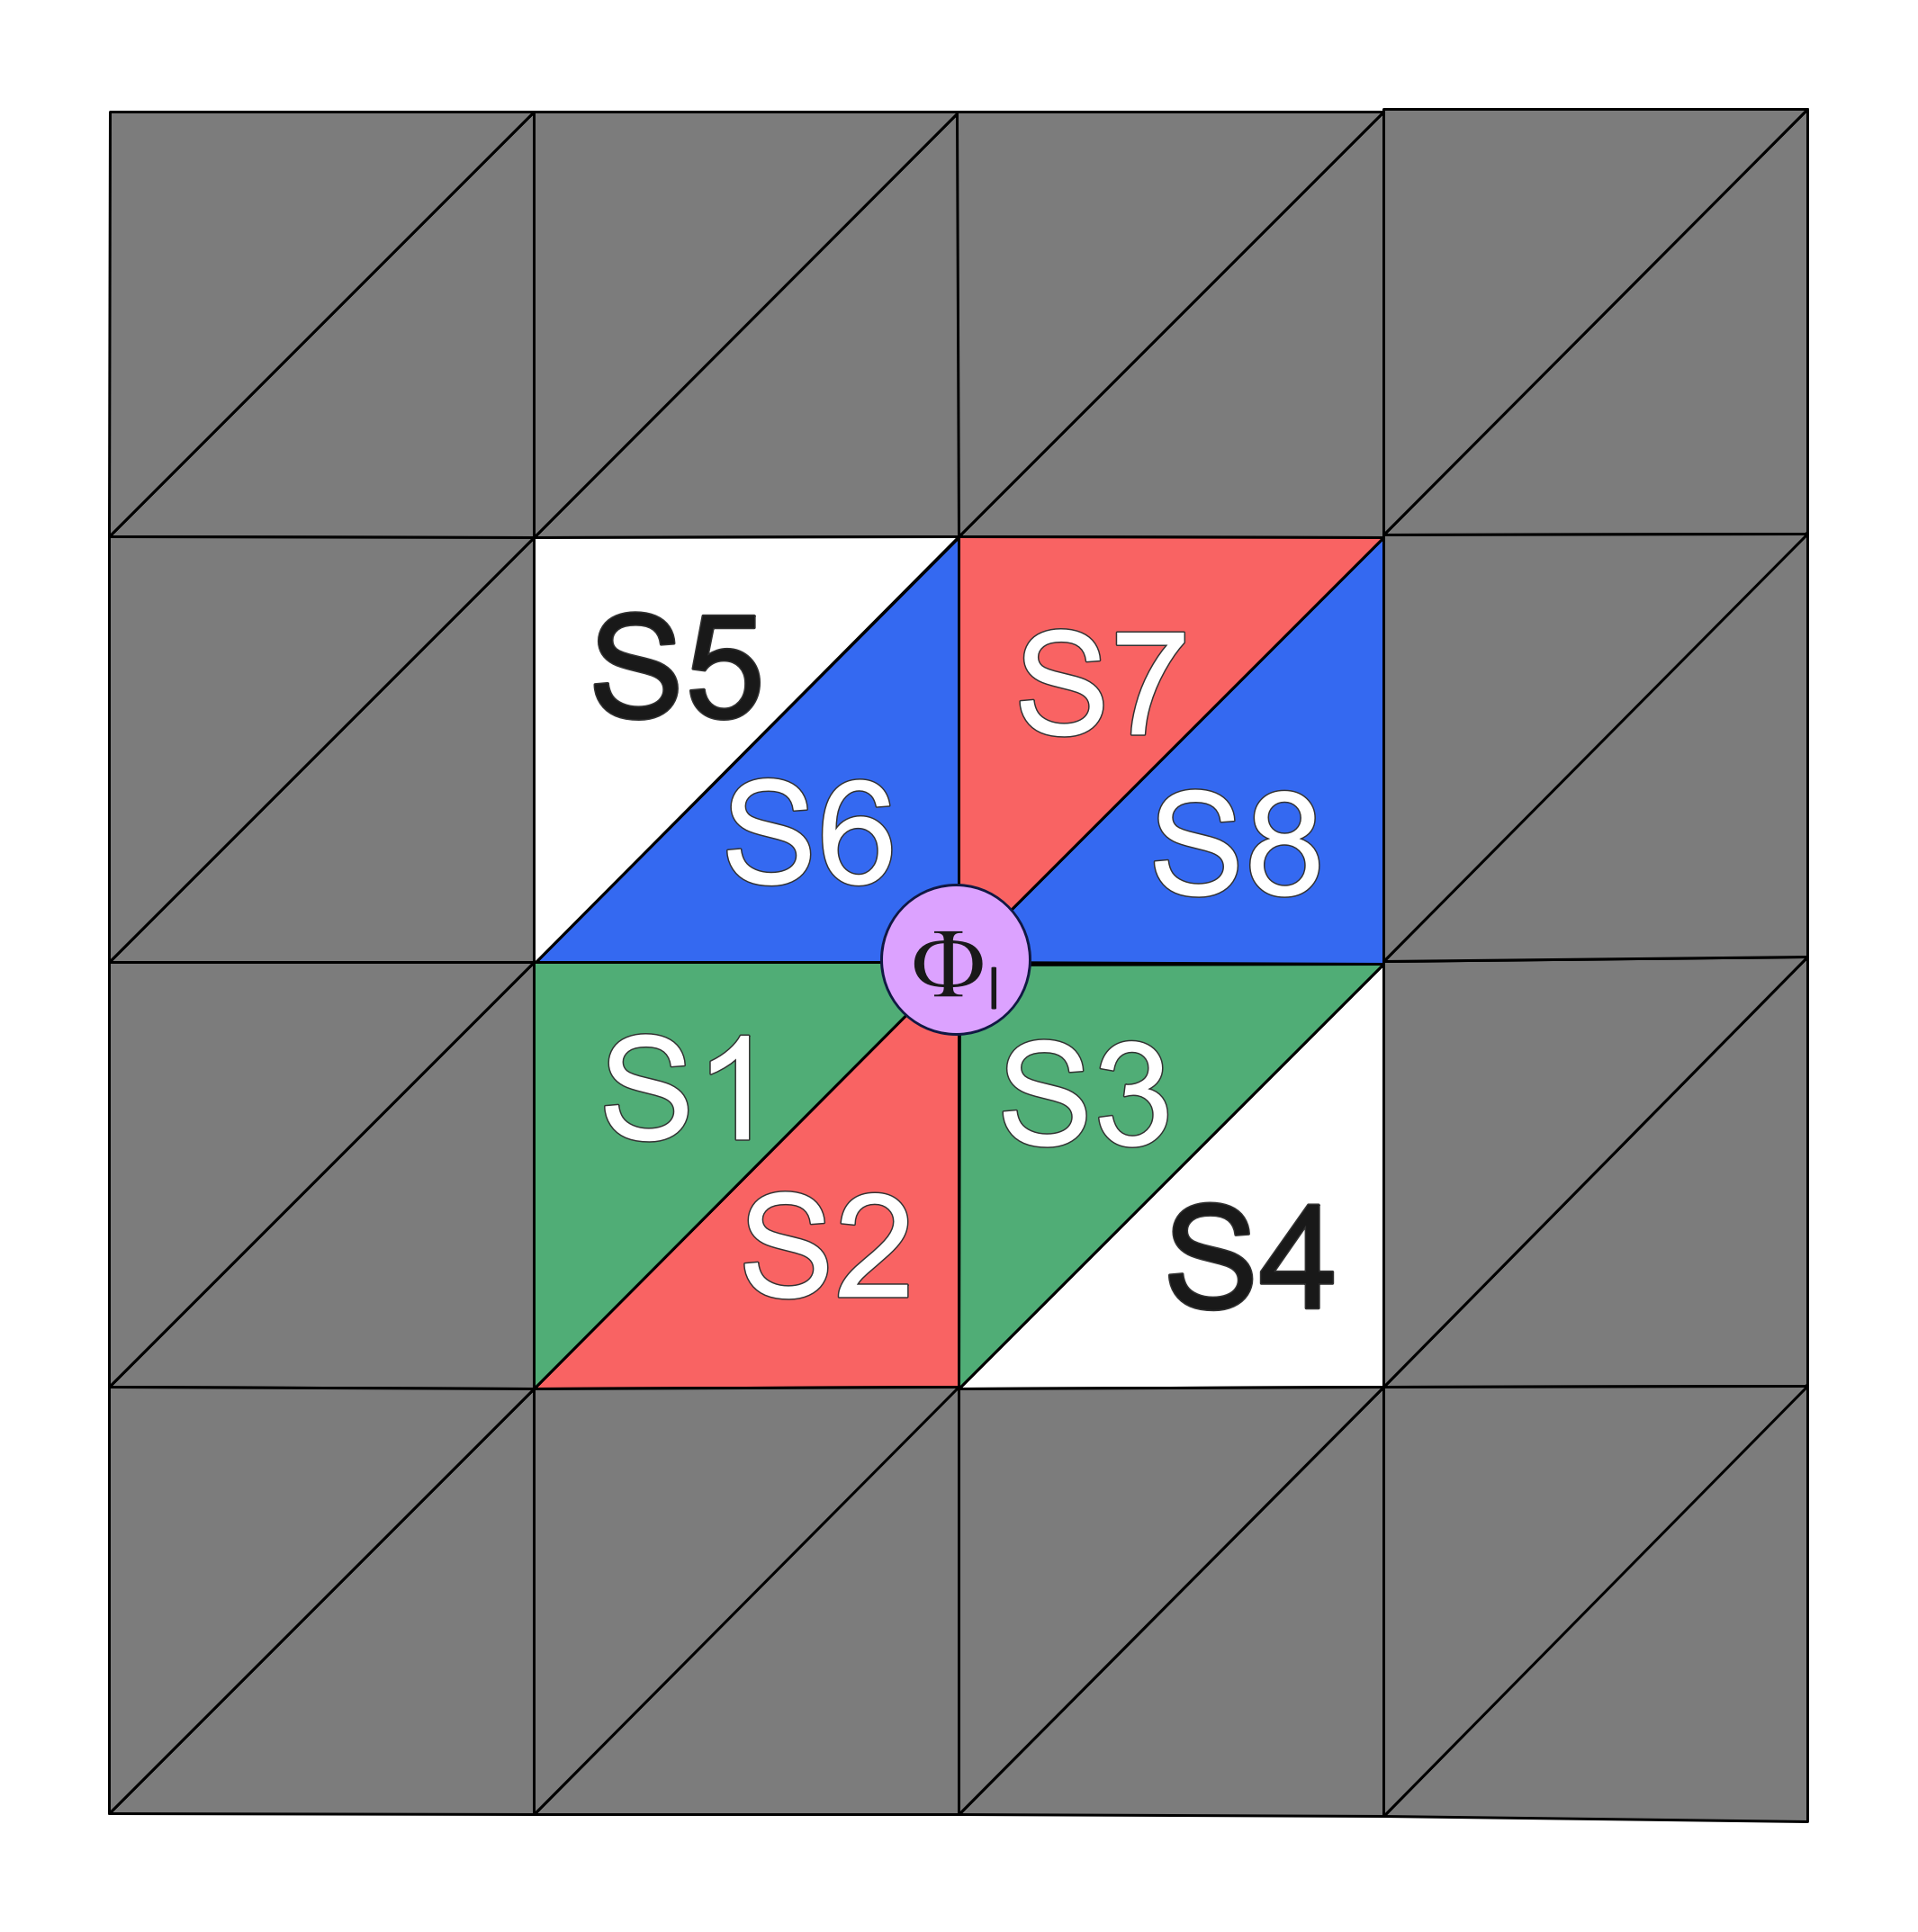
\includegraphics[scale=0.4]{./chapters/chapter2/figures/element.png}
\caption{
عناصر حول یک گره درونی شبکه مکانی.
}
\label{elementFig}
\end{figure}
در شکل
\ref{elementFig}
می‌توان نحوه شبکه‌بندی مثلثی یکنواخت بر بخشی از ناحیه
$\Omega$
را مشاهده کرد.
نحوه شماره‌گذاری عناصر از گوشه سمت چپ پایین ناحیه
$\Omega$
به‌صورت سطری و در راستای محور
$x$
است.

% ==========+==========+==========+==========+==========+==========+==========+==========
\chapter*{نتیجه‌گیری و پیشنهادات}
\addcontentsline{toc}{chapter}{نتیجه‌گیری و پیشنهادات}
\thispagestyle{empty}
% ==========+==========+==========+==========+==========
معادله
\eng{SFD} 
یک مسئله چالشی با کاربردهایی در مدل‌سازی انتشار غیرعادی، بررسی پدیده‌های زیرانتشار و توصیف دینامیک‌های آشوبی است.
چالش اصلی در حل عددی این معادله، غیرموضعی بودن عملگر کسری است که به تولید یک دستگاه پر در گسسته‌سازی مکانی منجر می‌شود و حجم محاسبات در هر گام زمانی را افزایش می‌دهد.
از طرفی با توجه به تعریف مشتق کسری، دقت محاسبات مربوط به هر درایه این دستگاه خود یک مشکل جدی است.
%\chapter*{پیوست‌ 1}
\thispagestyle{empty}\fancyhead[LE]{\nouppercase\thepage\ \hfill\ پیوست ۱}
\fancyhead[LO]{\nouppercase پیوست ۱ \ \hfill\ \thepage}
\addcontentsline{toc}{chapter}{پیوست‌ 1}
در این بخش الگوریتم‌های مورد نیاز در فصل ۳ رساله که به وسیله‌ی نرم‌ افزار GAP نوشته شده‌اند ارائه شده است. 
خروجی الگوریتم  Prog-I علاوه بر آن زیرمجموعه‌های سه عضوای از $\mathbb{Z}_n $ که  گراف کیلی جمعی حاصل همبند و صحیح است، 
قدرمطلق مقادیر ویژه‌ی گراف مذکور  نیز است. 
 
\hspace{1cm}
\begin{latin}
\noindent \bf Prog-I:
\end{latin}
$------------------------------------------$
\begin{code}
Main:=function(n)
local i,j,k,r,t,a,c,w,A,B,G,T,D;
G:=CyclicGroup(IsPermGroup,n);
a:=MinimalGeneratingSet(CyclicGroup(IsPermGroup,n))[1];
T:=Elements(List(G,x->x^2));     B:=Set([]);
for i in [1..n-1] do
  for j in [i+1..n-1] do
    for k in [j+1..n-1] do
      w:=0; A:=[]; D:=[];
      for r in [0..n-1] do
        c:=E(n)^(i*r)+E(n)^(j*r)+E(n)^(k*r);
        t:=ImaginaryPart(c)^2+RealPart(c)^2;
        if IsInt(t)  and IsInt(Sqrt(t)) then   w:=w+1;
        fi;
      od;
      if w=n and Intersection([a^i,a^j,a^k],T)=[]
         and Group(a^i,a^j,a^k)=G
         and Size(Group(a^(i-j),a^(i-k),a^(j-k)))>=Size(G)/2
      then
         Add(D,i); Add(D,j); Add(D,k); Add(A,D);
         for r in [0..n-1] do
           c:=E(n)^(i*r)+E(n)^(j*r)+E(n)^(k*r);
           t:=ImaginaryPart(c)^2+RealPart(c)^2;
           if IsInt(t) then  t:=Sqrt(t);
           fi;
           Add(A,t);
         od;
         Add(B,A);
      fi;
    od;
  od;
od;
return B;
end;
\end{code}
%\chapter*{پیوست‌ 2}
\thispagestyle{empty}\fancyhead[LE]{\nouppercase\thepage\ \hfill\ پیوست ۲}
\fancyhead[LO]{\nouppercase   پیوست ۲ \ \hfill\ \thepage}
\addcontentsline{toc}{chapter}{پیوست‌ 2}

  سرشت‌های تحویل ناپذیر دو گروه  $A_4$ و  $S_4$ به ترتیب در جدول‌های  Table-I  و Table-II ارائه شده است که در آن‌ها $C_G(g)$ مرکزساز عضو $g$ در گروه $G$ است. 
\label{p1}

\begin{latin}
\noindent \bf Table-I: 
\end{latin}
$------------------------------------------$
\begin{latin}
\begin{center} 
\begin{tabular}{c|cccc} 
\hline
$g_i$             &  $1$     &  $(1~2)(3~4)$   &  $(1~2~3)$   &   $(1~3~2)$  \\
$|C_G(g_i)|$   &  $12$   &   $4$                 &  $3$              &  $3$             \\
\hline 
$\chi_1$         &  $1$     &  $1$   &  $1$      &    $1$        \\
$\chi_2$         &  $1$     &  $1$   &  $w$      &  $w^2$     \\
$\chi_3$         &  $1$     &  $1$   &  $w^2$  &   $w$        \\
$\chi_4$         &  $3$     &  $-1$  &  $0$       &  $0$         \\

\hline
\end{tabular}
\end{center}
\end{latin}

\begin{latin}
\noindent \bf Table-II:
\end{latin}
$------------------------------------------$
\begin{latin}
\begin{center} 
\begin{tabular}{c|ccccc} 
\hline
$g_i$              &  $1$     &   $(1~2)$    & $(1~2~3)$    &    $(1~2)(3~4)$    &   $(1~2~3~4)$  \\
$|C_G(g_i)|$   &  $24$   &   $4$           &  $3$              &           $8$            &  $4$         \\
\hline 
$\chi_1$         &  $1$     &  $1$   &  $1$      &  $1$     &   $1$   \\
$\chi_2$         &  $1$     &  $-1$  &  $1$      &  $1$     &   $-1$     \\
$\chi_3$         &  $2$     &  $0$   &  $-1$     &  $2$     &   $0$       \\
$\chi_4$         &  $3$     &  $1$   &  $0$      &  $-1$    &   $-1$          \\
$\chi_5$         &  $3$     &  $-1$  &  $0$      &  $-1$    &   $1$        \\
\hline
\end{tabular}
\end{center}
\end{latin}
% ==========+==========#==========+==========#==========+==========#==========+==========#==========+==========
\renewcommand{\bibname}{\per{کتاب‌نامه}}
\fancyhead[LO]{\nouppercase\rightmark\ \hfill\ \thepage}
%%%%%%%%%%%%%%%%%%%%%%%%%%%%%%%%%%%%%%%%%%%%%%%%%%%%%%%%%%%%%%%%%%%%%%%%%%%%%%%%%%%%%%%%%%%%%%%%%%%%%%%%%%%%%%%%%%%%%%%%%%%%%
%%%%%%%%%%%%%%%%%%%%%%%%%%%%%%%%%%%%%%%%%%%%%%%%%%%%%%%%%%%%%%%%%%%%%%%%%%%%%%%%%%%%%%%%%%%%%%%%%%%%%%%%%%%%%%%%%%%%%%%%%%%%%
%%%%%%%%%%%%%%%%%%%%%%%%%%%%%%%%%%%%%%%%%%%%%%%%%%%%%%%%%%%%%%%%%%%%%%%%%%%%%%%%%%%%%%%%%%%%%%%%%%%%%%%%%%%%%%%%%%%%%%%%%%%%%
%%%%%%%%%%%%%%%%%%%%%%%%%%%%%%%%%%%%%%%%%%%%%%%%%%%%%%%%%%%%%%%%%%%%%%%%%%%%%%%%%%%%%%%%%%%%%%%%%%%%%%%%%%%%%%%%%%%%%%%%%%%%%

\begin{latin}

\begin{thebibliography}{99}
\thispagestyle{empty}
%\begin{latin}
%===============+===============
\bibitem{Ref28BSYXZ}
Bu, W. P., Shu, S., Yue, X. Q., Xiao, A. G., \& Zeng, W.  
(2019).
Space–time finite element method for the multi-term time-space fractional diffusion equation on a two-dimensional domain.
\textit{Comput. Math. Appl., 78}.
1367–1379.

%===============+===============
\bibitem{Ref21BTY}
Bu, W. P., Tang, Y. F., \& Yang, J. Y.
(2014).
Galerkin finite element method for two-dimensional Riesz space fractional diffusion equations.
\textit{J. Comput. Phys., 276}.
26–38.

%===============+===============
\bibitem{Ref24BTWY}
Bu, W. P., Tang, Y. F., Wu, Y. C., \& Yang, J. Y.
(2015).
Crank–Nicolson ADI Galerkin finite element method for two-dimensional fractional FitzHugh–Nagumo monodomain model.
\textit{Appl. Math. Comput., 257}.
355–364.

%===============+===============
\bibitem{Ref48CLZ}
Chen, H., Lv, W., \& Zhang, T. T.
(2018).
A Kronecker product splitting preconditioner for two-dimensional space-fractional diffusion equations.
\textit{J. Comput. Phys., 360}.
1–14.

%===============+===============
\bibitem{Ref15CDL}
Cheng, X. J., Duan, J. Q., \& Li, D. F.
(2019).
A novel compact ADI scheme for two-dimensional Riesz space fractional nonlinear reaction–diffusion equations.
\textit{Appl. Math. Comput., 346}.
452–464.

%===============+===============
\bibitem{Ref4DXL}
Ding, Z., Xiao, A., \& Li, M.
(2010).
Weighted finite difference methods for a class of space fractional partial differential equations with variable coefficients.
\textit{Journal of Computational and Applied Mathematics, 233}(8).
1905-1914.

%===============+===============
\bibitem{Ref57DKPS}
Dobrev, V. A., Kolev, Tz.,  Petersson, N. A., \& Schroder, J. B. 
(2017).
Two-level convergence theory for multigrid reduction in time (MGRIT).
\textit{SIAM Journal on Scientific Computing, 39}(5).
S501–S527.

%===============+===============
\bibitem{Ref20ER}
Ervin, V. J., \& Roop, J. P.
(2006).
Variational formulation for the stationary fractional advection dispersion equation.
\textit{Numer. Methods Partial Differential Equations, 22}.
558–576.

%===============+===============
\bibitem{Ref113E}
Evans, L. C.
(2010).
\textit{Partial differential equations} (2nd Ed.).
AMS.

%===============+===============
\bibitem{Ref52FFKMS}
Falgout, R. D., Friedhoff, S., Kolev, T. V., Maclachlan, S. P., \& Schroder, J. B.
(2012).
Parallel time integration with multigrid.
\textit{SIAM Journal on Scientific Computing, 36}(6).
635–661.

%===============+===============
\bibitem{Ref103FLW}
Falgout, R. D., Lecouvez, M., \& Woodward, C. S.
(2019).
A parallel-in-time algorithm for variable step multistep methods.
\textit{Journal of Computational Science, 37}.
101029.

%===============+===============
\bibitem{Ref105FMOS}
Falgout, R. D., Manteuffel, T. A., O'Neill, B., \& Schroder, J. B.
(2017).
Multigrid reduction in time for nonlinear parabolic problems: a case study
\textit{SIAM Journal on Scientific Computing, 39}(5).
S298-S322.

%===============+===============
\bibitem{Ref112FZLTG}
Feng, L. B., Zhuang, P., Liu, F., Turner, I., \& Gu, Y. T.
(2016).
Finite element method for space-time fractional diffusion equation
\textit{Numerical Algorithms, 72}.
749-767.

%===============+===============
\bibitem{Ref14FZLTAL}
Feng, L. B., Zhuang, P., Liu, F., Turner, I., Anh, V., \& Li, J.
(2017).
A fast second-order accurate method for a two-sided space-fractional diffusion equation with variable coefficients.
\textit{Computers \& Mathematics with Applications, 73}(6).
1155-1171.

%===============+===============
\bibitem{Ref108FW}
Fox, W. P., \& West, R. D.
(2025).
\textit{Numerical methods and analysis with mathematical modelling}.
CRC Press.

%===============+===============
\bibitem{Ref101FFKMS}
Friedhoff, S., Falgout, R. D., Kolev, T. V., Maclachlan, S. P., \& Schroder, J. B.
(2014).
A multigrid-in-time algorithm for solving evolution equations in parallel.
\textit{Lawrence Livermore National Laboratory}.

%===============+===============
\bibitem{Ref61G}
Gander, M. J.
(2015).
50 years of time parallel time integration.
\textit{Contrib. Math. Comput. Sci., 9}.
69–114.

%===============+===============
\bibitem{Ref55GV}
Gander, M. J., \& Vandewalle, S.
(2007).
Analysis of the Parareal Time Parallel Time Integration Method.
\textit{SIAM Journal on Scientific Computingm, 29}(2).
556-578.

%===============+===============
\bibitem{Ref107G}
Gockenbach, G. S.
(2006).
\textit{Understanding and implementing the finite element method}.
SIAM.

%===============+===============
\bibitem{Ref49GBT}
Gong, C. Y., Bao, W. M., \& Tang, G. J.
(2013).
A parallel algorithm for the Riesz fractional reaction–diffusion equation with explicit finite difference method.
\textit{Fract. Calc. Appl. Anal., 16}.
654–669.

%===============+===============
\bibitem{Ref42GBTJL}
Gong, C. Y., Bao, W. M., Tang, G. J., Jiang, Y. W., \& Liu, J.
(2015).
Computational challenge of fractional differential equations and the potential solutions: a survey.
\textit{Math. Probl. Eng., 2015}.
258–265.

%===============+===============
\bibitem{Ref114GGS}
Günther, S., Gauger, N. R., \&  Schroder, J. B.
(2018).
A non-intrusive parallel-in-time adjoint solver with the XBraid library.
\textit{Comput. Visual Sci., 19}.
85–95.

%===============+===============
\bibitem{Ref9HFCS}
Hao, Z. P., Fan, K., Cao, W. R., \& Sun, Z. Z. 
(2016).
A finite difference scheme for semilinear space-fractional diffusion equations with time delay.
\textit{Appl. Math. Comput., 275}.
238–254.

%===============+===============
\bibitem{Ref0HSNRFS}
Hessenthaler, A., Southworth, B. S., Nordsletten, D., R\"{o}hrle, O., Falgout, R. D., \& Schroder, J. B.
(2020).
Multilevel convergence analysis of Multigrid reduction-in-time.
\textit{SIAM Journal on Scientific Computing, 42}(2).
A771-A796.

%===============+===============
\bibitem{Ref63Hypre}
HYPRE: Scalable linear solvers and multigrid methods, 
\href{https://llnl.gov/casc/hypre}{\cod{https://llnl.gov/casc/hypre}}.

%===============+===============
\bibitem{Ref31JW}
Jia, J. H., \& Wang, H.
(2016).
A fast finite volume method for conservative space-fractional diffusion equations in convex domains.
\textit{J. Comput. Phys., 310}.
63–84.

%===============+===============
\bibitem{Ref109J}
Jin, B.
(2021).
\textit{Fractional differential equations: an approach via fractional derivatives}.
Springer.

%===============+===============
\bibitem{Ref51LMT}
Lions, J. L., Maday, Y., \& Turinici, G.
Résolution D’EDP par un schéma en tempspararéel.
\textit{C. R. Math. Acad. Sci. Paris 332}.
(2001).
661–668.

%===============+===============
\bibitem{Ref30LZTBA}
Liu, F., Zhuang, P., Turner, I., Burrage, K., \& Anh, V.
(2014).
A new fractional finite volume method for solving the fractional diffusion equation.
\textit{Appl. Math. Model., 38}.
3871–3878.

%===============+===============
\bibitem{Ref59N}
Nievergelt, J.
(1964).
Parallel methods for integrating ordinary differential equations.
\textit{Commun. ACM, 7}.
731–733.

%===============+===============
\bibitem{Ref43PS}
Pang, H. K., \& Sun, H. W.
(2012).
Multigrid method for fractional diffusion equations.
\textit{J. Comput. Phys., 231}.
693–703.

%===============+===============
\bibitem{Ref111R}
Reddy, B. D.
(1998).
\textit{Introductory functional analysis: with applications to boundary value problems and finite elements}.
Springer.

%===============+===============
\bibitem{Ref106RTW}
Ries, M., Trottenberg, U., \& Winter, G.
(1983).
A note on MGR methods.
\textit{Linear Algebra and its Applications, 49}.
1–26.

%===============+===============
\bibitem{Ref33SX}
Song, F. Y.,\& Xu, C. J.
(2015).
Spectral direction splitting methods for two-dimensional space fractional diffusion equations.
\textit{J. Comput. Phys., 299}.
196–214.

%===============+===============
\bibitem{Ref100SB}
Stoer, J., \& Bulirsch, R.
(2002).
\textit{Introduction to Numerical Analysis} (3rd ed.).
Springer.

%===============+===============
\bibitem{Ref110SG}
Sun, Z. Z., \& Gao, G. H.
(2020).
\textit{Fractional differential equations: Finite difference methods}.
De Gruyter.

%===============+===============
\bibitem{Ref102TMV}
Tielen, R., Möller, M., \& Vuik, C.
(2022).
Combining p-multigrid and MGRIT methods to obtain a scalable solver for Isogeometric Analysis.
\textit{SN Appl. Sci., 4}(163).

%===============+===============
\bibitem{Ref115TOS}
Trottenberg, U., Oosterlee, C., \& Schüller, A.
(2001).
\textit{Multigrid}. 
Academic Press, San Diego.

%===============+===============
\bibitem{Ref50WLGZX}
Wang, Q. L., Liu, J., Gong, C. Y., Zhang, Y., \& Xing, Z. C.
(2015).
A GPU-based fast solution for Riesz space fractional reaction–diffusion equation.
\textit{Proc. 18th Intl. Conf. Network-Based Info. Sys.}
317–323.

%===============+===============
\bibitem{Ref54WZ}
Wu, S. L., \& Zhou, T.
(2017).
Fast parareal iterations for fractional diffusion equations.
\textit{J. Comput. Phys., 329}.
210–226.

%===============+===============
\bibitem{Ref56XBraid}
XBraid: Parallel time integration with multigrid, 
\href{https://llnl.gov/casc/xbraid}{\cod{https://llnl.gov/casc/xbraid}}.

%===============+===============
\bibitem{Ref104XZ}
Xu, J., \& Zikatanov, L.
(2017).
Algebraic multigrid methods.
\textit{Acta Numerica, 26}.
591–721.

%===============+===============
\bibitem{Ref34Y}
Yang, Y.
(2015).
Jacobi spectral Galerkin methods for fractional integro-differential equations.
\textit{Calcolo, 52}.
519–542.

%===============+===============
\bibitem{Ref25YYNWZL}
Yang, Z., Yuan, Z., Nie, Y., Wang, J., Zhu, X., \& Liu, F.
(2019).
Finite element method for nonlinear Riesz space fractional diffusion equations on irregular domains.
\textit{J. Comput. Phys., 330}.
863–883.

%===============+===============
\bibitem{Ref0YSXBP}
Yue, X., Shu, S., Xu, X., Bu, W., \& Pan, K.
(2019).
Parallel-in-time multigrid for space–time finite element approximations of two-dimensional space-fractional diffusion equations.
\textit{Comput. Math. Appl., 78}.
3471–3484.

%===============+===============
\bibitem{Ref21BTYRef29ZLA}
Zhang, H., Liu, F., \& Anh, V.
(2010).
Galerkin finite element approximation of symmetric space-fractional partial differential equations
\textit{Appl. Math. Comput., 217}.
2534-2545.

%===============+===============
\bibitem{Ref26ZBZT}
Zhao, Y., Bu, W. P., Zhao, X., \& Tang, Y. F.
(2017).
Galerkin finite element method for two-dimensional space and time fractional Bloch-Torrey equation.
\textit{J. Comput. Phys., 350}.
117–135.

%===============+===============
%\end{latin}

\end{thebibliography}

\end{latin}

%%%%%%%%%%%%%%%%%%%%%%%%%%%%%%%%%%%%%%%%%%%%%%%%%%%%%%%%%%%%%%%%%%%%%%%%%%%%%%%%%%%%%%%%%%%%%%%%%%%%%%%%%%%%%%%%%%%%%%%%%%%%%%%%%%%%%%%%%%%%%%%%%%%%%%%%%%%%%%%%%%%%%%%%%%%%%%%%%%%%%%%%%%%%%%%%%%%%%%%%%%%%%%%%%%%%%%%%%%%%%%%%%%%%%%%%%%%%%%%%%%%%%%%%%%%%%%%%%%%%%%%%%%%%%%%%%%%%%%%%%%%%%%%%%%%%%%%%%%%%%%%%%%%%%%%%%%%%%%%%%%%%%%%%%%%%%%%%%%%%%%%%%%%%%%%%%%%%%%%%%%%%%%%%%%%%%%%%%%%%%%%%%%%%%%%%%%%%%%%%%%%%%%%%%%%%%%%%%%%%%%%%%%%%%%%%%%%%%%%%%%%%%%%%%%%%%%%%%%%%%%%%%%%%%%%%%%%%%%%%%%%%%%%%%%%%%%%%%%%%%%%%%%%%%%%%%%%%%%%%%%%%%%%%%%%%%%%%%%%%%%%%%%%%%%%%%%%%%%%%%%%%%%%%%%%%%%%%%%%%%%%%%%%%%%%%%%%%%%%%%%%%%%%%%%%%%%%%%%%%%%%%%%%%%%%%%%%%%%%%%%%%%%%%%%%%%%%%%%%%%%%%%%%%%%%%%%%%%%%%%%%%%%
 
% ==========+==========#==========+==========#==========+==========#==========+==========#==========+==========
\cleardoublepage
\parindent=0pt
\fancyhead[LO]{\nouppercase  واژه‌نامه فارسی به انگلیسی  \ \hfill\ \thepage}
%
\chapter*{واژه‌نامه فارسی به انگلیسی}
\thispagestyle{empty}
%\fancyhead[LO]{\nouppercase واژه‌نامه فارسی به انگلیسی \ \hfill\ \thepage}
%\fancyhead[LE]{\nouppercase واژه‌نامه فارسی به انگلیسی \ \hfill\ \thepage}
%\lhead{\thepage}\rhead{واژه‌نامه‌ی فارسی به انگلیسی}
%\fancyhead[LO]{\nouppercase\thepage\ \hfill\ واژه‌نامه فارسی به انگلیسی}
%\fancyhead[LO]{\nouppercase\rightmark\ \hfill\ \thepage}
\addcontentsline{toc}{chapter}{واژه‌نامه فارسی به انگلیسی}
%%%%%%
{\bf ا}
\vspace*{3mm}

\farsiTOenglish{اساسی}{Underlying}
\farsiTOenglish{انتشاردهنده زمانی}{Temporal propagator}

{\bf پ}
\vspace*{3mm}

\farsiTOenglish{پیشرو}{Marching}

{\bf ت}
\vspace*{3mm}
    
\farsiTOenglish{توأم}{Simultaneous}
\farsiTOenglish{توزیع‌یافته}{Distributed}    

{\bf چ}
\vspace*{3mm}
    
\farsiTOenglish{چندجمله‌ای‌های قطعه‌ای}{Piecewise polynomials}
\farsiTOenglish{چرخه}{Cycle}

{\bf د}
\vspace*{3mm}

\farsiTOenglish{درشت}{Coarse}
\farsiTOenglish{درون‌یاب سراسری}{Global interpolation}
\farsiTOenglish{درون‌یاب موضعی}{Local interpolation}
\farsiTOenglish{دوخطی}{Bilinear}

{\bf ر}
\vspace*{3mm}

\farsiTOenglish{رایانه خوشه‌ای}{Cluster computer}

{\bf ز}
\vspace*{3mm}

\farsiTOenglish{زبرینه اساسی}{Essential supremum}
\farsiTOenglish{زیرانتشار}{Subdiffusion}

{\bf س}
\vspace*{3mm}

\farsiTOenglish{سلسله مراتب}{Hierarchy}

{\bf ش}
\vspace*{3mm}

\farsiTOenglish{شبکه}{Mesh, Grid}

{\bf ظ}
\vspace*{3mm}

\farsiTOenglish{ظریف}{Fine}

{\bf ف}
\vspace*{3mm}

\farsiTOenglish{فراواقعی}{Parareal}
\farsiTOenglish{فضای آزمایش}{Test Space}
\farsiTOenglish{فضای آزمون}{Trial Space}

{\bf ق}
\vspace*{3mm}

\farsiTOenglish{قطری‌‌شونده توأم}{Simultaneous diagonalization}
  
{\bf ک}
\vspace*{3mm}

\farsiTOenglish{کاهش کلی}{Total-reduction}
\farsiTOenglish{کاهش تناوبی}{Alternating-reduction}

{\bf م}
\vspace*{3mm}

\farsiTOenglish{محدودیت}{Restriction}
\farsiTOenglish{محمل}{Support}
\farsiTOenglish{مقیاس‌پذیر}{Scalabe}

{\bf و}
\vspace*{3mm}

\farsiTOenglish{وادارنده}{Coercive}

{\bf ه}
\vspace*{3mm}

\farsiTOenglish{همروندسازی}{Concurrency}
\farsiTOenglish{هموار}{Smooth}
      % check label of last page
\fancyhead[LO]{\nouppercase  واژه‌نامه فارسی به انگلیسی  \ \hfill\ \thepage}

\cleardoublepage
\parindent=0pt
\fancyhead[LO]{\nouppercase  واژه‌نامه انگلیسی به فارسی  \ \hfill\ \thepage}

\chapter*{واژه‌نامه انگلیسی به فارسی}
\thispagestyle{empty}
\addcontentsline{toc}{chapter}{واژه‌نامه انگلیسی به فارسی}
%%%%%%
\begin{flushleft}
{\bf A}
\end{flushleft}
\vspace*{2mm}

\englishTOfarsi{Affine}{ آفین}
\englishTOfarsi{Analytic function}{تابع تحلیلی}


\begin{flushleft}
{\bf B}
\end{flushleft}
\vspace*{2mm}

\englishTOfarsi{Boundary component}{مولفه مرزی}

\begin{flushleft}
{\bf C}
\end{flushleft}
\vspace*{2mm}

\englishTOfarsi{Calculation}{محاسبات}
\englishTOfarsi{Center}{مرکز}
\englishTOfarsi{Change}{تبدیل}
\englishTOfarsi{Closed orbit}{مدار بسته}
\englishTOfarsi{Coefficient}{ضریب}
\englishTOfarsi{Compactness}{فشردگی}
\englishTOfarsi{Continuous}{پیوسته}
\englishTOfarsi{Contradiction}{تناقض}
\englishTOfarsi{Coordinates}{مختصات}
\englishTOfarsi{Corollary}{نتیجه}
\englishTOfarsi{Counted with multiplicities}{با احتساب تکرار}
\englishTOfarsi{Criteria}{معیار}
\englishTOfarsi{Critical period}{دوره بحرانی}
\englishTOfarsi{Curve}{منحنی}

\begin{flushleft}
	{\bf D}
\end{flushleft}
\vspace*{3mm}

\englishTOfarsi{Dehomogenized}{غیرهمگن}
\englishTOfarsi{Denominator}{مخرج}
\englishTOfarsi{Divid}{تقسیم}
\englishTOfarsi{Discriminant}{مبین}


\begin{flushleft}
	{\bf E}
\end{flushleft}
\vspace*{3mm}

\englishTOfarsi{Energy level}{سطح انرژی}
\englishTOfarsi{Explicit}{صریح}

\begin{flushleft}
	{\bf F}
\end{flushleft}
\vspace*{3mm}

\englishTOfarsi{Factor}{عامل}
\englishTOfarsi{First integral}{انتگرال اول}
\englishTOfarsi{Foliated}{افراز (یا ورقه‌بندی) شده }
\englishTOfarsi{Function}{تابع}

\begin{flushleft}
{\bf H}
\end{flushleft}
\vspace*{3mm}

\englishTOfarsi{Hamiltonian system}{دستگاه همیلتونی}
\englishTOfarsi{Half-plane}{نیم‌صفحه}

\begin{flushleft}
{\bf I}
\end{flushleft}
\vspace*{3mm}

\englishTOfarsi{Implicitly}{به‌صورت ضمنی}
\englishTOfarsi{Integrating factor}{عامل انتگرال‌ساز}
\englishTOfarsi{Interval}{بازه}
\englishTOfarsi{Invariant}{ناوردا}
\englishTOfarsi{Involution}{برگردان}
\englishTOfarsi{Isochronous}{هم‌زمان-هم‌دوره}

\begin{flushleft}
	{\bf L}
\end{flushleft}
\vspace*{3mm}

\englishTOfarsi{Lemma}{لم}

\begin{flushleft}
	{\bf M}
\end{flushleft}
\vspace*{3mm}

\englishTOfarsi{Multiplicities}{چندگانگی‌ها}
\englishTOfarsi{Maple}{میپل}
\englishTOfarsi{Mapping}{نگاشت}
\englishTOfarsi{Maximum}{بیشینه}
\englishTOfarsi{Minimum}{کمینه}
\englishTOfarsi{Monotone}{یکنوا}
\englishTOfarsi{Monotonicity}{یکنوایی}
\englishTOfarsi{Multiply}{ضرب}

\begin{flushleft}
	{\bf N}
\end{flushleft}
\vspace*{3mm}

\englishTOfarsi{Negative}{منفی}
\englishTOfarsi{Neighborhood}{همسایگی}
\englishTOfarsi{Notation}{نماد}

\begin{flushleft}
	{\bf P}
\end{flushleft}
\vspace*{3mm}

\englishTOfarsi{Parameter}{پارامتر}
\englishTOfarsi{Period annulus}{طوق تناوبی}
\englishTOfarsi{Period annuli}{طوق‌های تناوبی}
\englishTOfarsi{Period function}{تابع دوره تناوب}
\englishTOfarsi{Polynomial}{چند‌جمله‌ای}
\englishTOfarsi{Polycycle}{چندسیکل}
\englishTOfarsi{Potential system}{دستگاه پتانسیل}
\englishTOfarsi{Procedure}{روش}
\englishTOfarsi{Proof}{اثبات}
\englishTOfarsi{Proposition}{گزاره}
\englishTOfarsi{Punctured}{محذوف}

\begin{flushleft}
	{\bf R}
\end{flushleft}
\vspace*{3mm}

\englishTOfarsi{Regular}{ منظم}
\englishTOfarsi{Rescaling}{تغییرمقیاس}
\englishTOfarsi{Resultant}{برآیند}
\englishTOfarsi{Reversible}{برگشت‌پذیر}
\englishTOfarsi{Root}{ریشه}

\begin{flushleft}
{\bf S}
\end{flushleft}
\vspace*{3mm}

\englishTOfarsi{Sign}{علامت}
\englishTOfarsi{Statement}{گزاره}
\englishTOfarsi{Surrounding}{حول}

\begin{flushleft}
{\bf T}
\end{flushleft}
\vspace*{3mm}

\englishTOfarsi{Tangent}{مماس}
\englishTOfarsi{Theorem}{قضیه}
\englishTOfarsi{Transformation}{تبدیل}
\englishTOfarsi{True}{درست}

\begin{flushleft}
{\bf U}
\end{flushleft}
\vspace*{3mm}

\englishTOfarsi{Unique}{یکتا}

\begin{flushleft}
{\bf V}
\end{flushleft}
\vspace*{3mm}

\englishTOfarsi{Variation method}{روش تغییرات}



\begin{flushleft}
	{\bf W}
\end{flushleft}
\vspace*{3mm}

\englishTOfarsi{Well defined}{خوش‌تعریف}


 % check label of last page
\fancyhead[LO]{\nouppercase  واژه‌نامه انگلیسی به فارسی  \ \hfill\ \thepage}
% ==========+==========#==========+==========#==========+==========#==========+==========#==========+==========
%%%%%%%%%%%%%
\chapter*{فهرست نمادها}
\thispagestyle{empty}

\addcontentsline{toc}{chapter}{فهرست نمادها}

\symb{\text{نماد}}{مفهوم}{}

\symb{\Real}{اعداد حقیقی}{}
\symb{\RealP}{اعداد حقیقی مثبت}{}
\symb{\Natural}{اعداد طبیعی}{}
\symb{\Odd}{اعداد فرد}{}

   
\fancyhead[LO]{\nouppercase  فهرست نمادها  \ \hfill\ \thepage}
\cleardoublepage
\pagestyle{empty}
% ==========+==========#==========+==========#==========+==========#==========+==========#==========+==========
%%%%%%%%%%%%%
\chapter*{فهرست کلمات اختصاری}
\thispagestyle{empty}

\addcontentsline{toc}{chapter}{فهرست کلمات اختصاری}

\symbb{\text{اختصار}}{معنی}{کلمه کامل}

\symbb{\text{\eng{FEM}}}{روش عناصر متناهی (المان محدود)}{\eng{Finite elements method}}
\symbb{\text{\eng{FPDEs}}}{معادلات با مشتقات جزئی کسری}{\eng{Fractional partial differential equations}}
\symbb{\text{\eng{SFD}}}{انتشار کسری-مکانی}{\eng{Space-fractional diffusion}}
\symbb{\text{\eng{MGR}}}{کاهش چندشبکه‌ای}{\eng{Multigrid reduction}}
\symbb{\text{\eng{MGRIT}}}{کاهش در زمان چندشبکه‌ای}{\eng{Multigrid reduction-in-time}}

   
\fancyhead[LO]{\nouppercase  فهرست کلمات اختصاری  \ \hfill\ \thepage}
\cleardoublepage
\pagestyle{empty}
% ==========+==========#==========+==========#==========+==========#==========+==========#==========+==========
\fancyhead[LO]{\nouppercase\rightmark\ \hfill\ \thepage}
\fancyhead[LE]{\nouppercase\rightmark\ \hfill\ \thepage}
\renewcommand{\baselinestretch}{.9}
\latin
\tnr
\vskip -1.1cm
\begin{center}
\textbf{Multigrid reduction-in-time algorithms for solving fractional partial differential equations}
\\
\medskip
Ali Forouzandeh Hafshejani
\\
aforouzandeh@math.iut.ac.ir
\\
August 31, 2024
\\
Master of Science  Thesis (in Farsi)
\\
Departement of Mathematical Sciences
\\
Isfahan University of Technology, Isfahan 84156-8311, Iran
\end{center}
\vskip -5.5mm
\hrulefill
\\
\noindent
\textbf{Supervisor}: Dr. Reza Mokhtari, \texttt{mokhtari@iut.ac.ir}
\\
\textbf{Advisor}: Dr. Mohadese Ramezani, \texttt{mohadeseh.ramezani@alumni.iut.ac.ir}
\\
\textbf{2020 MSC}: 65M55, 65M60, 65Y05.
\\
\textbf{Keywords}: Fractional calculus, Space-fractional diffusion, FEM, Parallel-in-time, Multigrid reduction-in-time.  

\noindent
\hrulefill
\\
\textbf{Abstract:}
\\
{
\small 
This M.Sc. thesis is based on the following paper
\begin{itemize}\addtolength{\itemsep}{-0.4\baselineskip}
\item
Yue, X., Shu, S., Xu, X., Bu, W., \& Pan, K.
(2019).
Parallel-in-time multigrid for space–time finite element approximations of two-dimensional space-fractional diffusion equations.
\textit{Comput. Math. Appl., 78}.
3471–3484.
\end{itemize}
Nowadays, temporal or spatial fractional partial differential equations (FPDEs) have found applications in real-world problems in science and engineering. 
This popularity stems from the fractional derivative's nonlocal property compared to the local nature of the integer-order derivative. 
One of the most important FPDEs is the space-fractional diffusion equation (SFD) which has applications in modeling anomalous diffusion, investigating subdiffusive phenomena, and describing chaotic dynamics.
SFD over two-dimensional spaces is widely recognized as a key diffusion equation. 
It is derived from generalizing the spatial derivatives from integer order to fractional order within the partial differential equation. 
Since most SFD equations can not be solved analytically, various numerical methods, such as the finite difference method, local discontinuous Galerkin approach, and finite element method (FEM), have been proposed to achieve both high accuracy and efficiency.
It is important to note that fractional derivatives use global information, while classical derivatives rely on local information. 
As a result, regardless of the discretization method used, significant computational effort is required due to the nonlocality introduced by fractional differential operators. 
Many researchers have worked on developing fast algorithms to address this challenge. 
In addition to these rapid solutions, parallel computing approaches, such as multigrid reduction in time (MGRIT), should also be considered potential techniques. 
\\
In this thesis, we begin by discussing fundamental concepts in functional analysis, including vector spaces, function spaces, and Sobolev spaces, as well as the principles of fractional calculus. 
We explain that fractional derivatives and integrals are foundational to fractional calculus, with the Ritz fractional derivative being particularly favored for applications in spatial domains. 
Next, we examine various fractional spaces, such as fractional Sobolev spaces, and investigate their properties.
Additionally, we address spaces associated with FPDEs. 
\\
After that, we investigate the SFD problem with Dirichlet boundary conditions. 
We start by explaining the FEM and its properties. 
We construct the weak form of the SFD equation and apply space-time discretization, utilizing uniform spatial discretization and non-uniform temporal discretization. 
This process results in a large, sparse system of equations.
To solve the SFD equation numerically, we represent the method as a time-marching loop, where a spatial linear system is solved at each time step. 
This time-marching loop acts as a one-step temporal method, similar to solving a lower bidiagonal block system over time. 
We also discuss various schemes for temporal parallelization and provide a brief historical context.
One notable technique is MGRIT, which utilizes a multigrid reduction approach. 
The MGRIT offers two significant advantages: it minimizes interference with existing codes and allows optimal scalability. 
Subsequently, we employ a two-stage version of the MGRIT method to solve the lower bidiagonal system of the block unit and analyzing its convergence performance. 
\\
Finally, we implement a numerical example in MATLAB and XBraid and examine some tests. 
The results indicate that the method demonstrates adequate consistency and convergence for numerical solutions of such SFD equations, and it can be extended to solve some complicated FPDEs.
}














 
  
\Eapprovalpage %{برای تولید صفحه صورتجلسه انگلیسی دفاعیه  این دستور را فعال کنید}
\lastpage
% ==========+==========#==========+==========#==========+==========#==========+==========#==========+==========
\end{document}